\documentclass{beamer}
\usepackage[finnish]{babel}
\usepackage[T1]{fontenc}
\usepackage[utf8]{inputenc}
\usepackage{tikz}
\usetheme{Warsaw}
\title[Data-assimilaatio kitkamallissa]{Data-assimilaatio kitkamallissa}
\author{Tom Gustafsson}
\date{5. syyskuuta 2012}
\begin{document}

\begin{frame}
\titlepage
\end{frame}

\begin{frame}{Ongelma}

\begin{itemize}
\item Lähtökohtana: Onnistuuko huonosti tunnettujen parametrien ennustaminen elastisesta kitkamallista \emph{data-assimilaation} tarjoamien keinojen avulla?
\end{itemize}

\begin{figure}
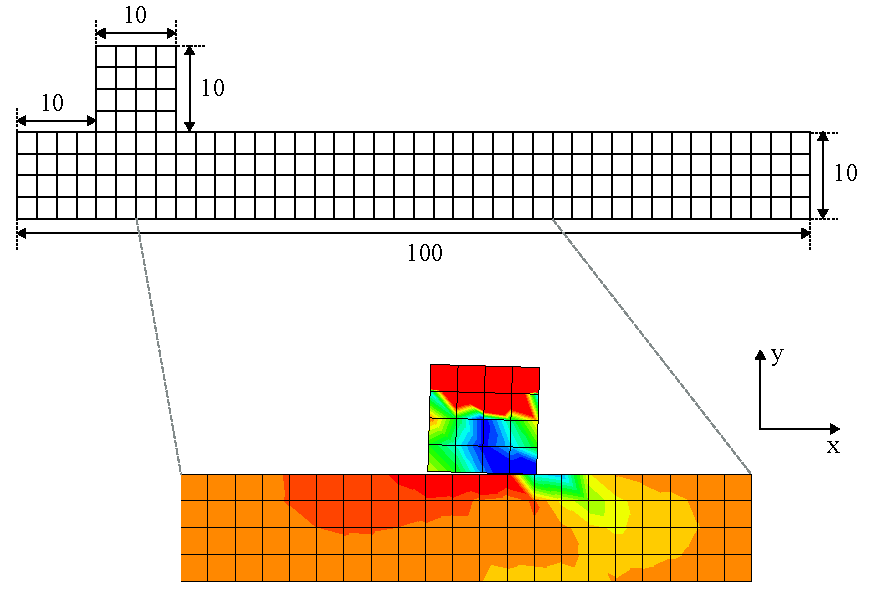
\includegraphics[width=8cm]{fretting_mesh.pdf}
\end{figure}

\end{frame}

\begin{frame}{Malli, 2D}

\begin{itemize}
\item Alkutila: Painin, laatta
\item Reunaehdot
\end{itemize}

\begin{figure}
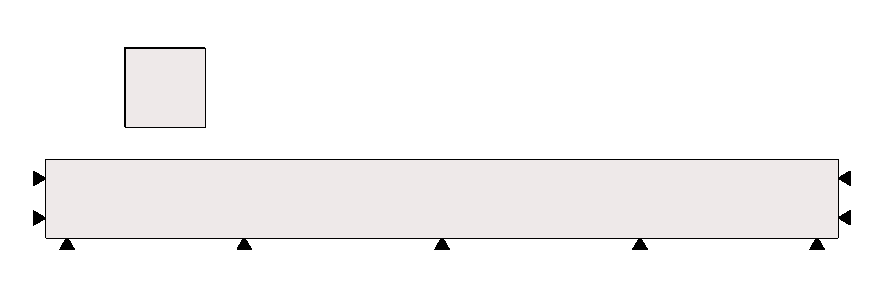
\includegraphics[width=10cm]{fretting_geom.pdf}
\end{figure}

\begin{itemize}
\item Abaqus/Standard 6.12-1, simulaatiot CSC:n koneella
\end{itemize}

\end{frame}

\begin{frame}{Simulaation vaiheet}

\begin{itemize}
\item Vaihe 1: 5 kN voima
\end{itemize}

\begin{figure}
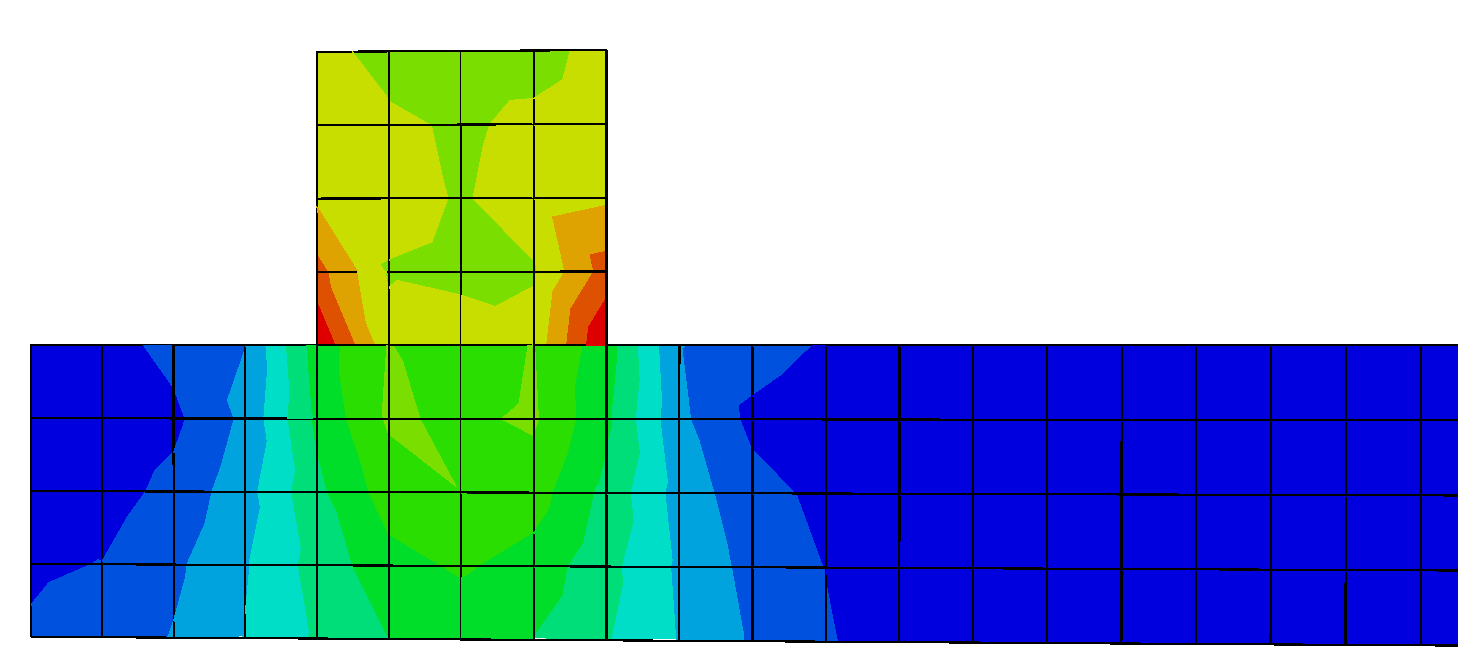
\includegraphics[width=9cm]{mises.pdf}
\end{figure}

\begin{itemize}
\item Vaihe 2: Yläreunan siirto 70 cm oikealle
\end{itemize}

\end{frame}

\begin{frame}{Simulaation vaiheet: Yläreunan siirtymä}

\begin{itemize}
\item Siirto reunaehdolla, ns. "hidas siirtymä"
\end{itemize}

\begin{figure}
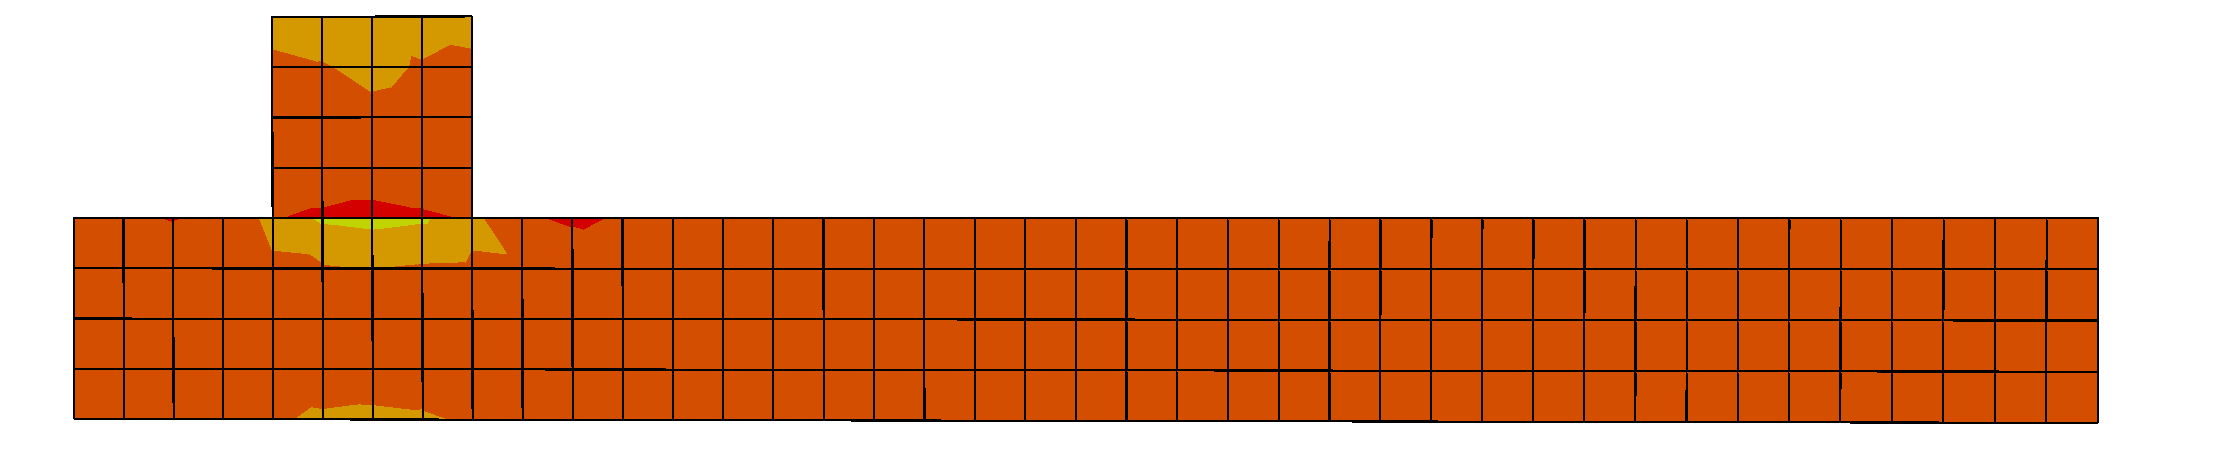
\includegraphics[width=10cm]{anim1.pdf}\\
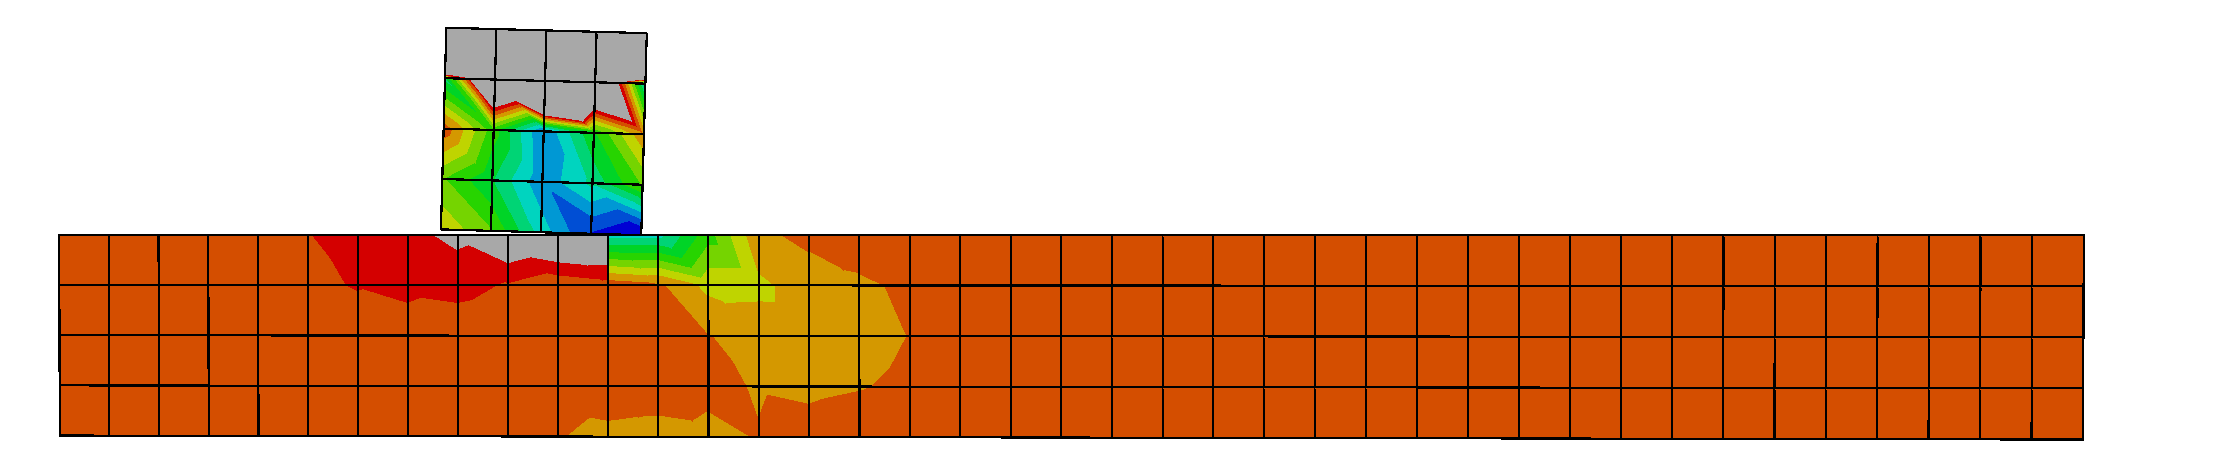
\includegraphics[width=10cm]{anim2.pdf}
\end{figure}

\end{frame}

\begin{frame}{Simulaation vaiheet: Yläreunan siirtymä 2}

\begin{figure}
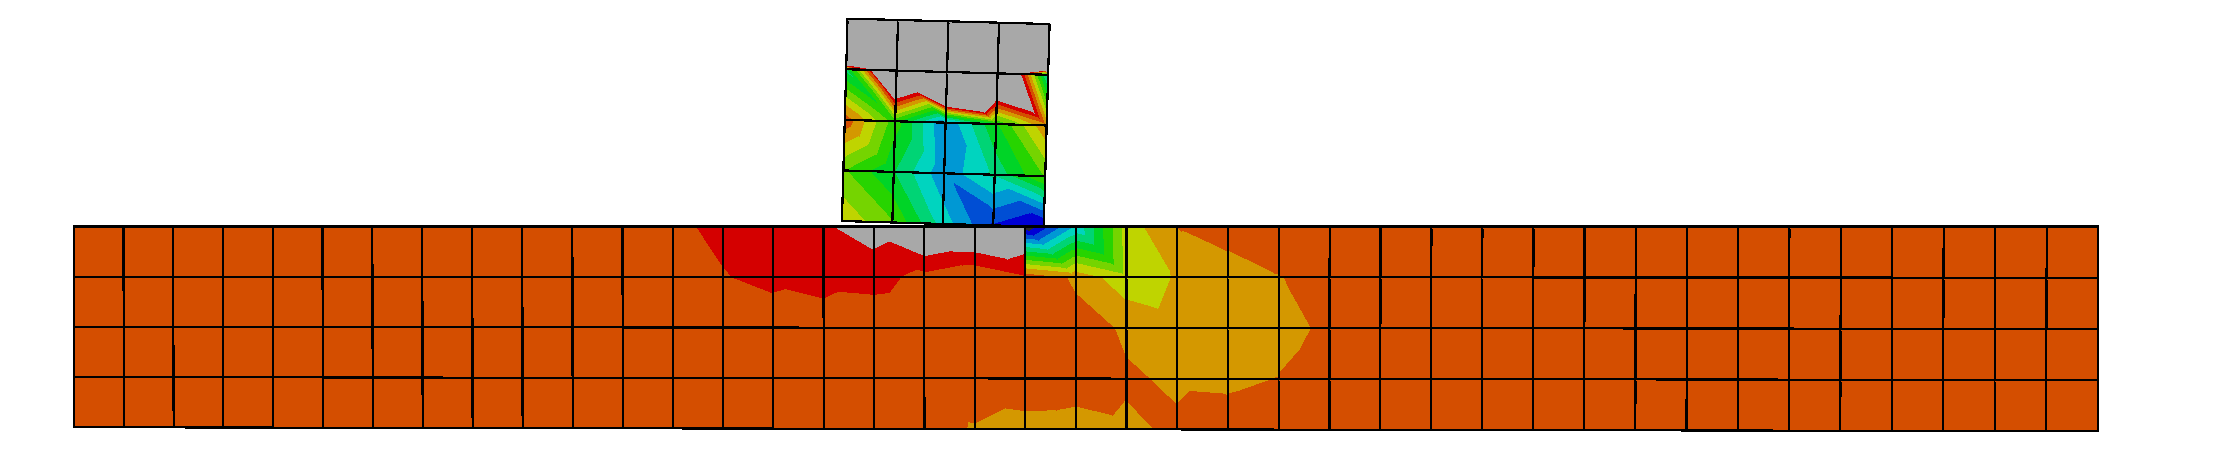
\includegraphics[width=10cm]{anim3.pdf}\\
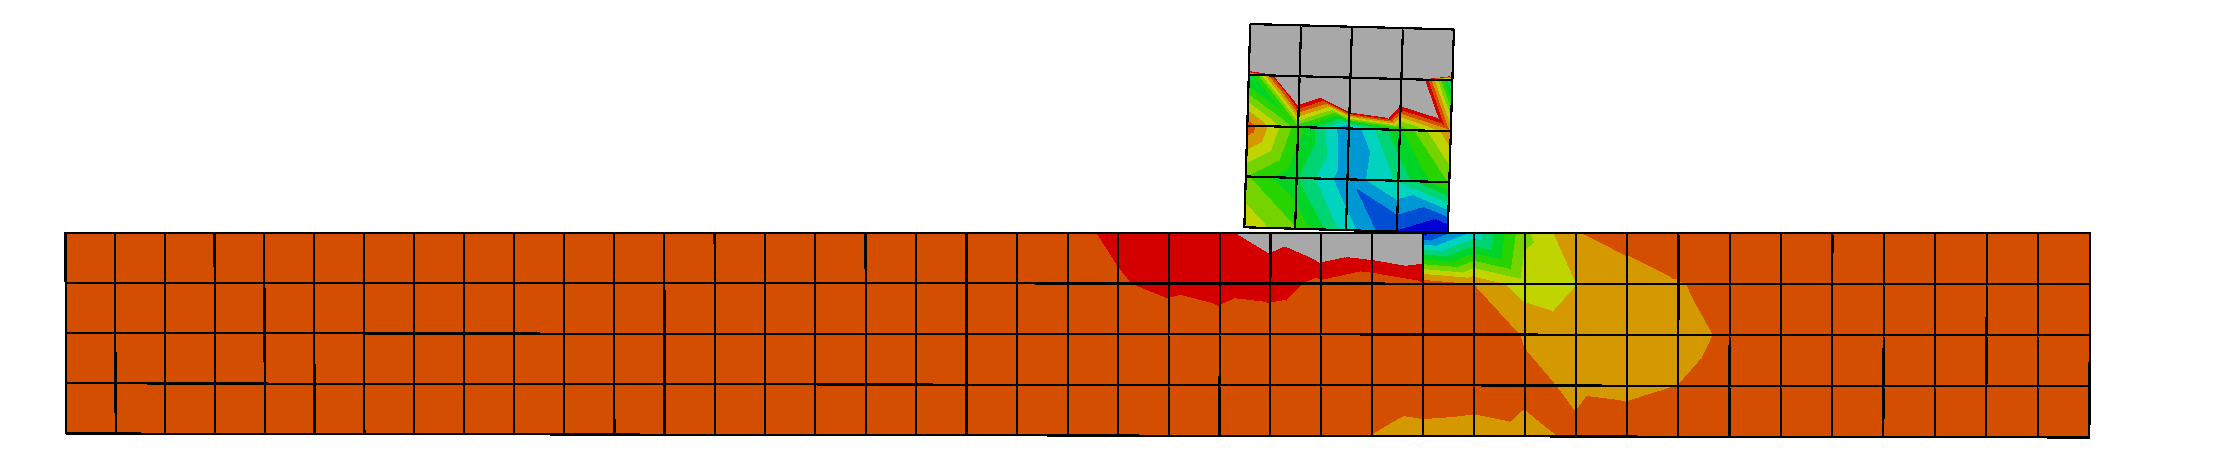
\includegraphics[width=10cm]{anim4.pdf}\\
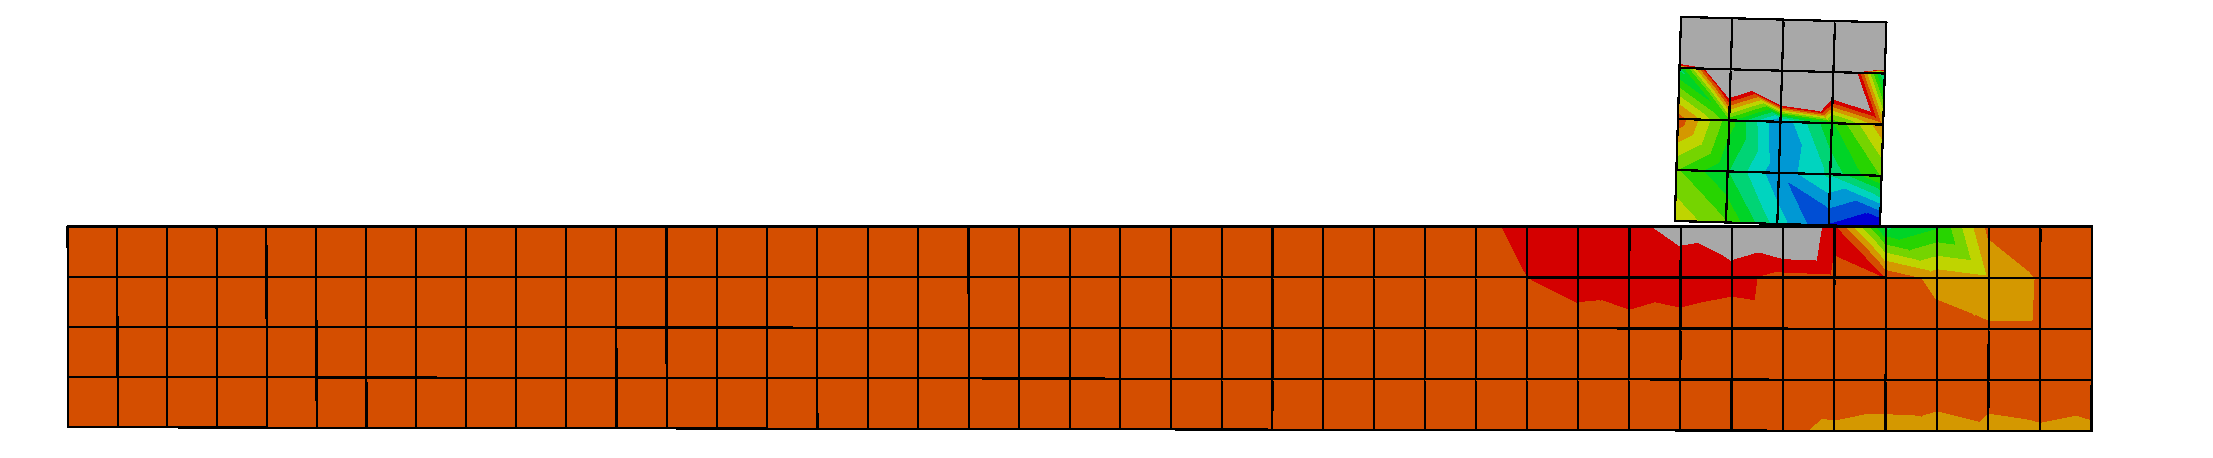
\includegraphics[width=10cm]{anim5.pdf}
\end{figure}

\end{frame}

\begin{frame}{Inversio-ongelma}

\begin{itemize}
\item Pyritään estimoimaan kitkakerroin $\mu$
\item Etukäteistietona $x$-suuntaiset jännitykset mittapisteissä\\($\sim$ venymäliuskamittaus)
\end{itemize}

\begin{figure}
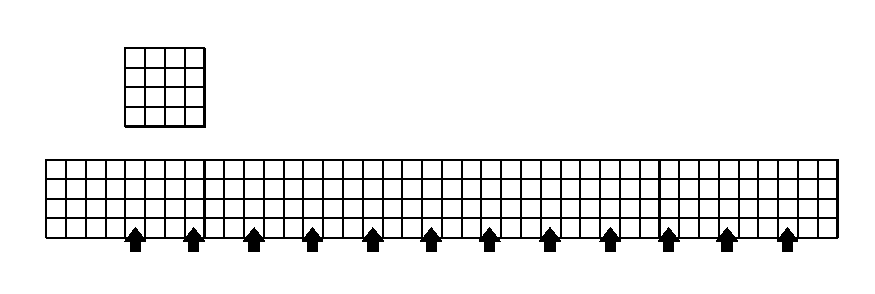
\includegraphics[width=10cm]{fretting_geom_meas.pdf}
\end{figure}

%\begin{itemize}
%\item Mittadata synteettistä
%\end{itemize}

\end{frame}

%\begin{frame}{Synteettisen mittadatan generointi}

%\begin{itemize}
%\item Minimoidaan inversiorikosta $\rightarrow$ mittadata tiheämmästä verkosta
%\end{itemize}

%\begin{figure}
%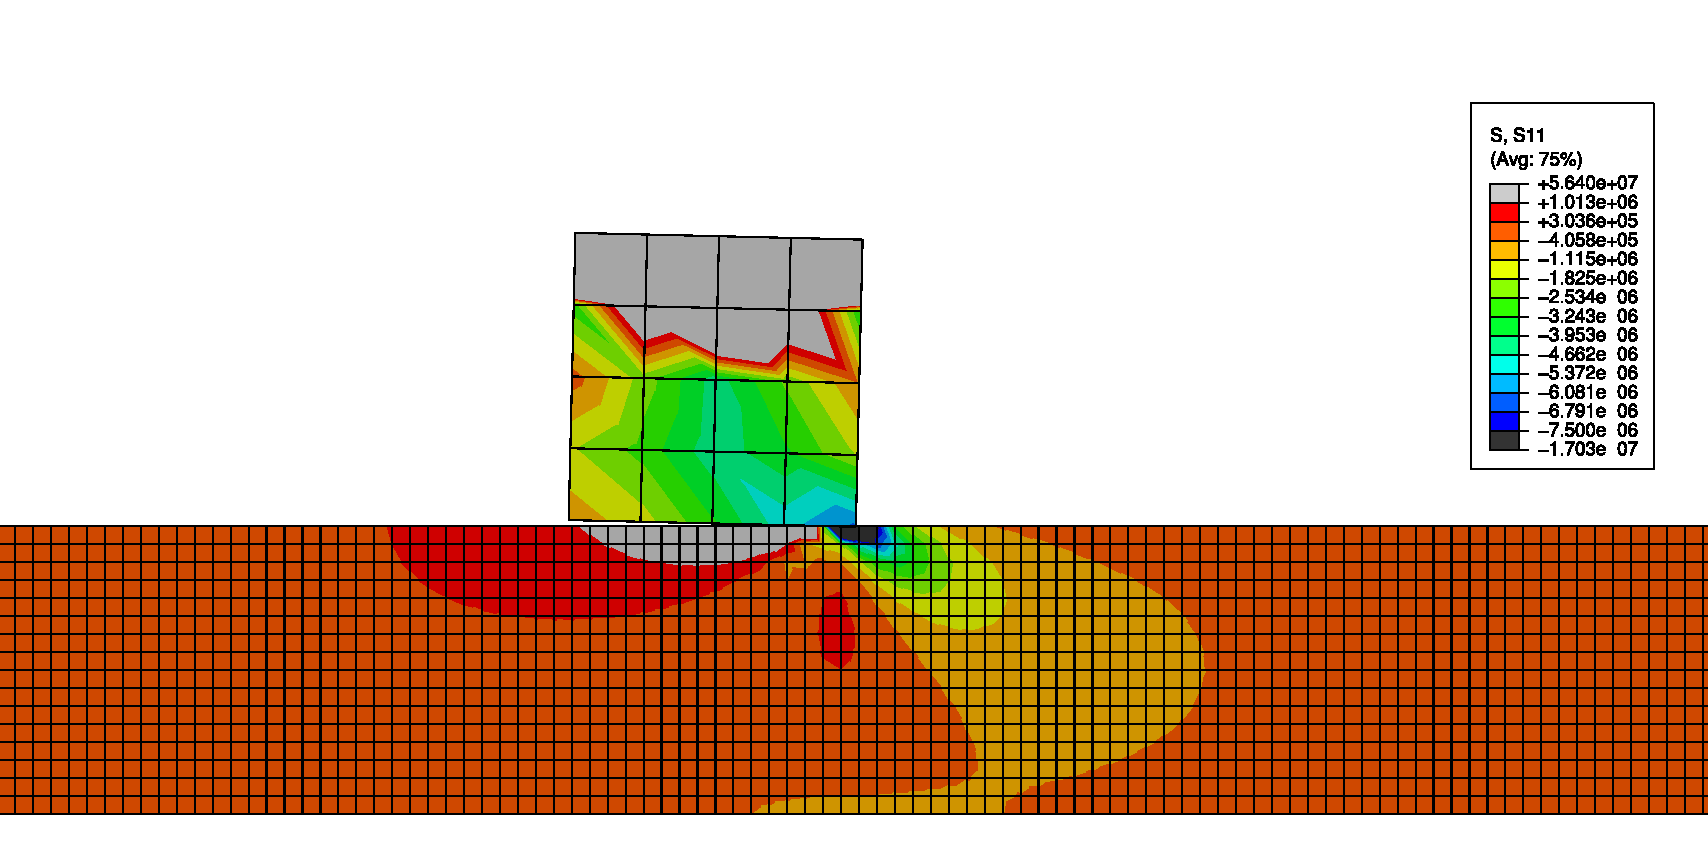
\includegraphics[width=10cm]{finer_mesh.pdf}
%\end{figure}

%\begin{itemize}
%\item Miten verrata tiheämmän ja harvemman verkon antamia jännityksiä?
%\end{itemize}

%\end{frame}

%\begin{frame}{Synteettisen mittadatan generointi 2}

%\begin{figure}
%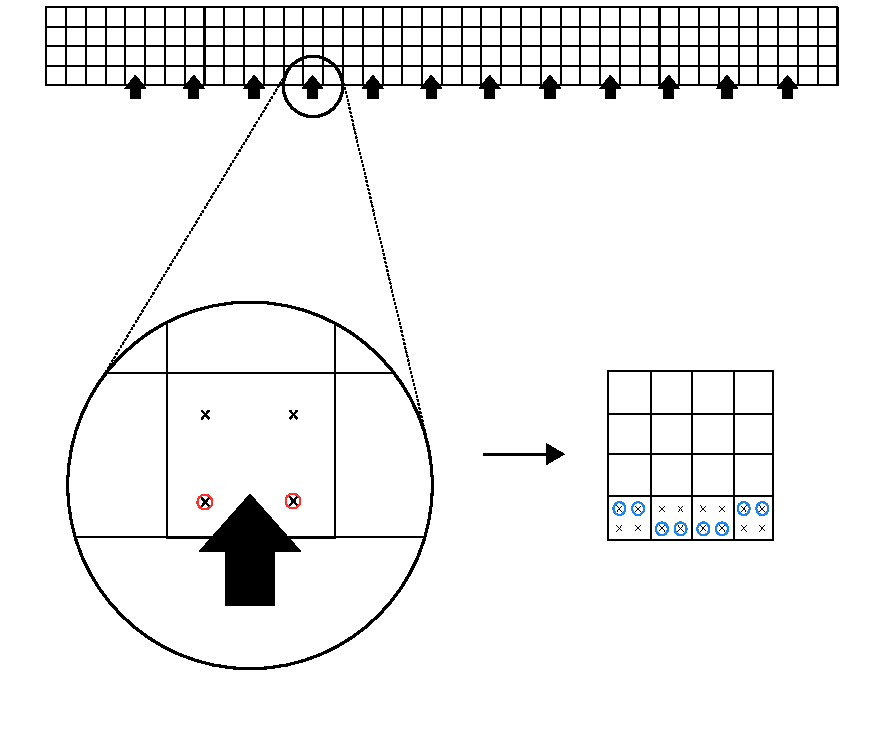
\includegraphics[width=10cm]{fretting_meas_tarkempi.pdf}
%\end{figure}

%\end{frame}

%\begin{frame}{Ongelman yhteenveto}

%\begin{itemize}
%\item Estimoitava suure: Kitkakerroin $\mu=0{,}5$
%\item Etukäteistieto: $x$-suuntaiset jännitykset mittapisteissä
%\item \emph{Data-assimilaatio}
%\end{itemize}

%\end{frame}

\begin{frame}{Ennen kuin jatketaan}

\begin{figure}
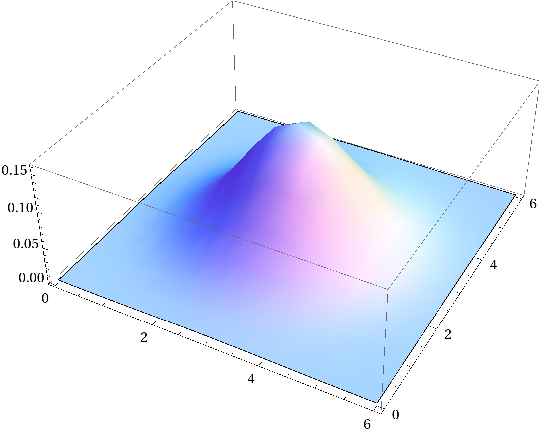
\includegraphics[width=5cm]{2dnormal.pdf}
$~~$
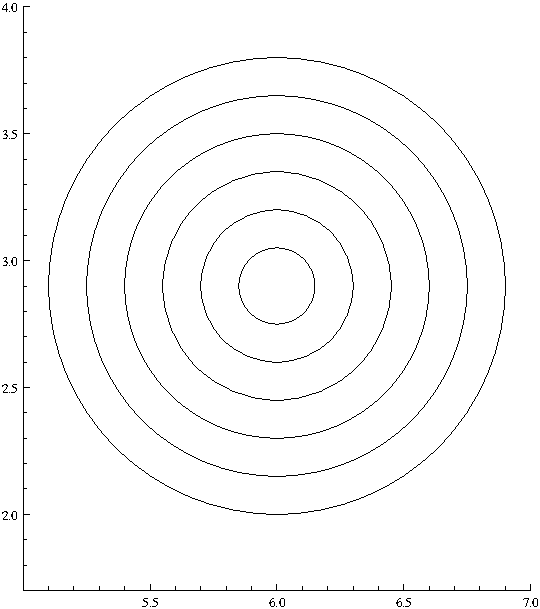
\includegraphics[width=5cm]{2dcontour.pdf}
\end{figure}

\end{frame}

\begin{frame}{Ennen kuin jatketaan 2}

\begin{itemize}
\item Useampiulotteisen normaalijakauman karakterisoi kovarianssimatriisi $\boldsymbol{\Sigma}$
\item $\mathcal{N}_k(\boldsymbol{\mu}_0,\boldsymbol{\Sigma})$, jossa $\boldsymbol{\Sigma} \in \mathbb{R}^{k \times k}$
\item Neliömatriisi, diagonaalilla varianssit eri dimensioissa
\item Muut alkiot kertovat dimensioiden välisen kovarianssin
\end{itemize}

\end{frame}

\begin{frame}{Data-assimilaatio}

\begin{itemize}
\item Pohjimmiltaan havaintojen ja mallin tuotaman informaation yhteensulauttamista
\item Perinteisiä sovelluskohteita: Säähavaintomallit, valtamerimallit
\item Data-assimilaation menetelmiä
\begin{itemize}
\item 3DVar, 4DVar
\item Kalman Filter, Extended-, Ensemble-, ...
\item ...
\end{itemize}
\item Tässä työssä \emph{Ensemble Kalman Filter}, eli EnKF
\end{itemize}

\end{frame}

\begin{frame}{Data-assimilaatio, yleistä}

\begin{itemize}
\item Systeemin (todellinen) tila $\boldsymbol{\psi}^t \in \mathbb{R}^N$
\item Mittaus $\boldsymbol{d} \in \mathbb{R}^M$
\begin{itemize}
\item Ei tarkka
\item Suhde tilaan $\boldsymbol{d} = \mathbf{M}\boldsymbol{\psi}^t+\boldsymbol{\epsilon}$
\item Mittamatriisi $\mathbf{M} \in \mathbb{R}^{M \times N}$
\item Virhe $\boldsymbol{\epsilon} \sim \mathcal{N}_M(0,\boldsymbol{\Sigma})$
\item Kovarianssimatriisi $\boldsymbol{\Sigma} \in \mathbb{R}^{M \times M}$
\end{itemize}
\item Ennustettu tila $\boldsymbol{\psi}^f \in \mathbb{R}^N$
\begin{itemize}
\item Aluksi esim. mittauksien perusteella
\end{itemize}
\end{itemize}

\end{frame}

\begin{frame}{Data-assimilaatio, yleistä 2}

\begin{itemize}
\item Todellinen tila $\boldsymbol{\psi}^t$ muuttuu ajan kuluessa
\item Systeemin malli
\[
\boldsymbol{\dot{\psi}} = \boldsymbol{G}(\boldsymbol{\psi},t)
\]
\item Aikakehitys:
\[
\boldsymbol{\psi}^f_{t+\Delta t} = \boldsymbol{\psi}^f_t + \int_{t}^{t+\Delta t} \! \boldsymbol{G}(\boldsymbol{\psi},t) \, \mathrm{d}t
\]
\begin{itemize}
\item Malli epätäydellinen, eli ennusteen virhe kasvaa aikakehitettäessä
\item Virheen kasvua kuvaa kovarianssimatriisi $\mathbf{Q}$
\end{itemize}
\end{itemize}

\end{frame}

\begin{frame}{Data-assimilaatio, esimerkki}

$N=M=2,~\mathbf{M} = \mathbf{I},~\boldsymbol{\Sigma} = \sigma\mathbf{I}$

\begin{figure}
\begin{tikzpicture}
\node[above right] (img) at (0,0) {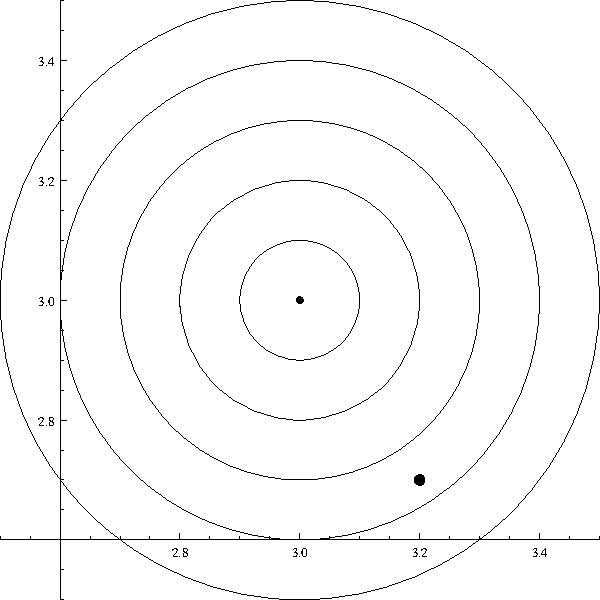
\includegraphics[width=6cm]{enkf1.pdf}};
\node at (100pt,90pt) {$\boldsymbol{\psi}^f_{t_0}$};
\node at (135pt,40pt) {$\boldsymbol{\psi}^t_{t_0}$};
\end{tikzpicture}
\end{figure}

\end{frame}

\begin{frame}{Data-assimilaatio, esimerkki 2}

\begin{figure}
\begin{tikzpicture}
\node[above right] (img) at (0,0) {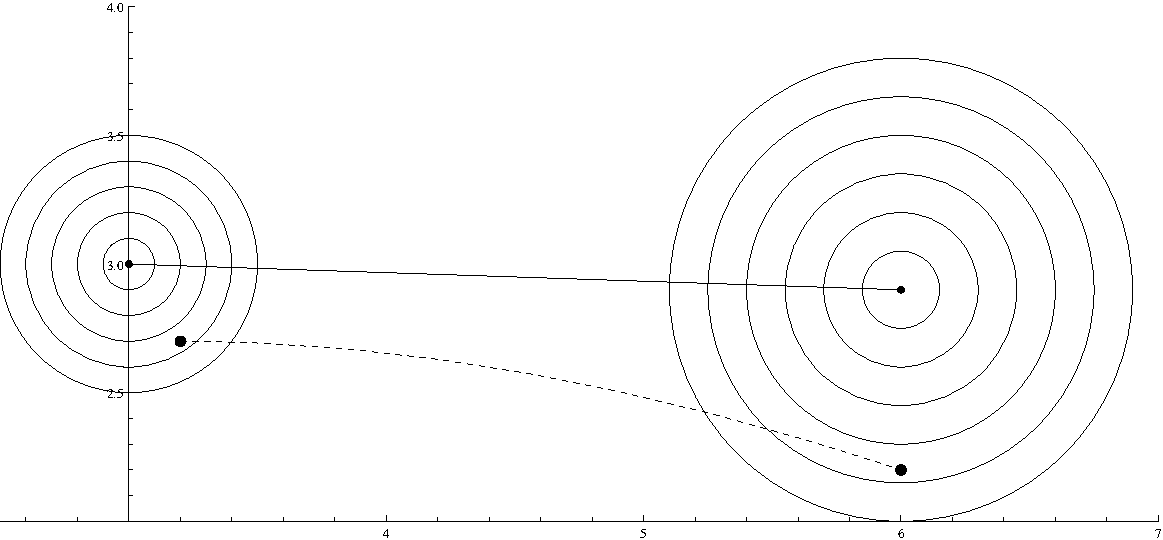
\includegraphics[width=11cm]{enkf2.pdf}};
\node at (47pt,86pt) {$\small \boldsymbol{\psi}^f_{t_0}$};
\node at (60pt,65pt) {$\small \boldsymbol{\psi}^t_{t_0}$};
\node at (255pt,80pt) {$\small \boldsymbol{\psi}^f_{t_1}$};
\node at (255pt,30pt) {$\small \boldsymbol{\psi}^t_{t_1}$};
\end{tikzpicture}
\end{figure}

\end{frame}

\begin{frame}{Data-assimilaatio, yleistä 3}

\begin{itemize}
\item Tulkitaan normaalijakauma todennäköisyystiheysfunktiona $f(\boldsymbol{\psi},t)$
\item Tällöin $f$:n aikakehitystä kuvaa \emph{Fokker-Planck -yhtälö}
\[
\frac{\partial f}{\partial t} + \sum_{i=1}^N \frac{\partial \left ( G_i f \right )}{\partial \psi_i} = \frac{1}{2} \sum_{i=1}^N \sum_{j=1}^N \frac{\partial^2 \left ( Q_{ij} f \right )}{\partial \psi_i \partial \psi_j}
\]
%\item \emph{Hurja}, mutta ei niin hurja miltä näyttää (sij. $\mathbf{G} = \mathbf{0}$ ja $\mathbf{Q} = \mathbf{I}$) 
\item Yleinen tapaus ei ratkea analyyttisesti $\rightarrow$ EnKF
\end{itemize}

\end{frame}

\begin{frame}{Ensemble Kalman Filter}

\begin{itemize}
\item Idea: Otetaan $n$-kappaletta realisaatioita alkutilan normaalijakaumasta ($\Rightarrow$ kokoelma)
\item Aikakehitetään näin saadun \emph{kokoelman} jokaista tilaa erikseen operaattorin $\boldsymbol{G}$ avulla
\item Tällöin ennusteen kovarianssimatriisia voidaan approksimoida lausekkeella
\[
\boldsymbol{\Sigma} \approx \frac{1}{n-1} \sum_{j=1}^n \left( \boldsymbol{\psi}^f_j - \overline{\boldsymbol{\psi}^f} \right) \left(\boldsymbol{\psi}^f_j - \overline{\boldsymbol{\psi}^f}  \right)^\mathrm{T}
\]
\end{itemize}

\end{frame}

\begin{frame}{Ensemble Kalman Filter, esimerkki}

\begin{figure}
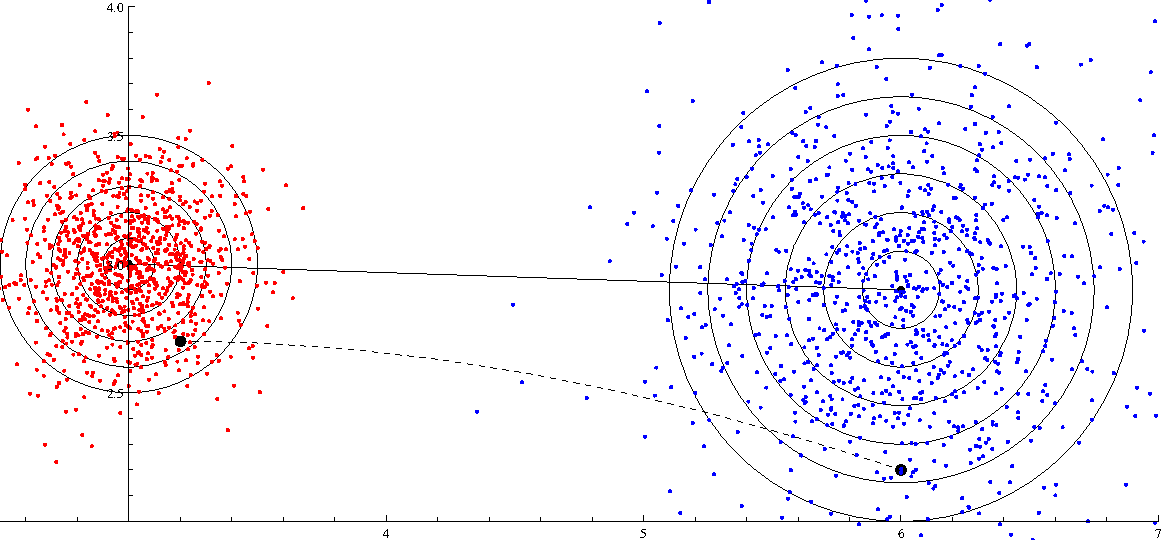
\includegraphics[width=11cm]{enkf3.pdf}
\end{figure}

\end{frame}

\begin{frame}{Ensemble Kalman Filter, esimerkki jatkuu}

\begin{figure}
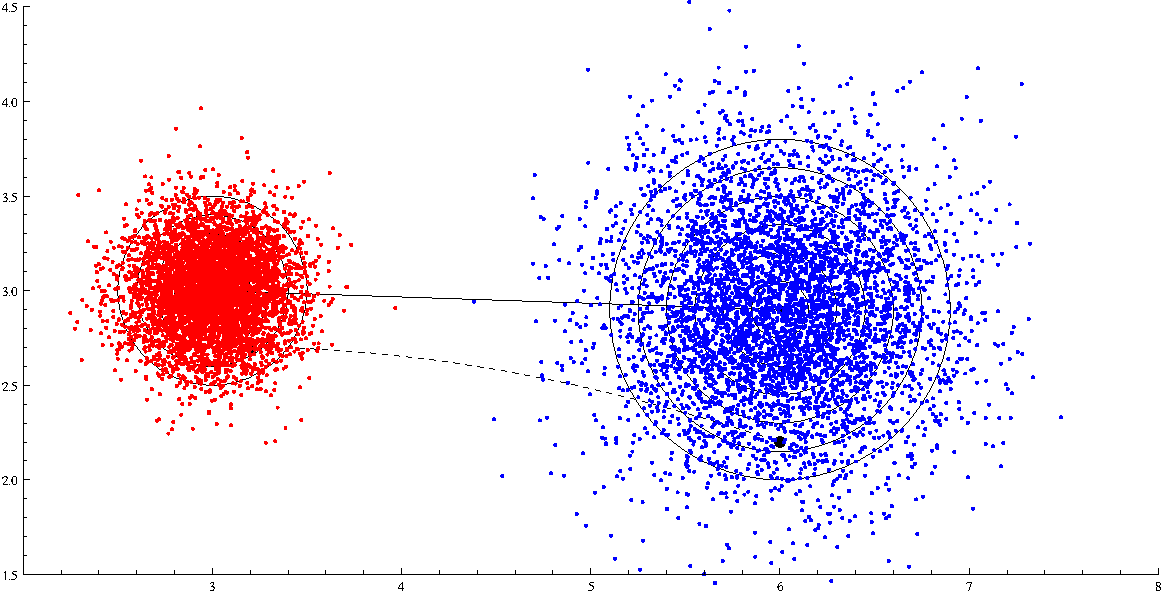
\includegraphics[width=11cm]{enkf4.pdf}
\end{figure}

\end{frame}

\begin{frame}{Ensemble Kalman Filter, analyysiongelma}

\begin{itemize}
\item Tyypillisesti systeemistä saadaan mittadataa mittahetkillä $t_1, t_2, t_3, \dots$
\item Analyysiongelma: \emph{Miten yhdistää optimaalisesti mallin ennuste $\boldsymbol{\psi}^f$ ja uusi mittaus $\boldsymbol{d}$?}
\end{itemize}

\end{frame}

\begin{frame}{Ensemble Kalman Filter, analyysiongelma 2}

\begin{figure}
\begin{tikzpicture}
\node[above right] (img) at (0,0) {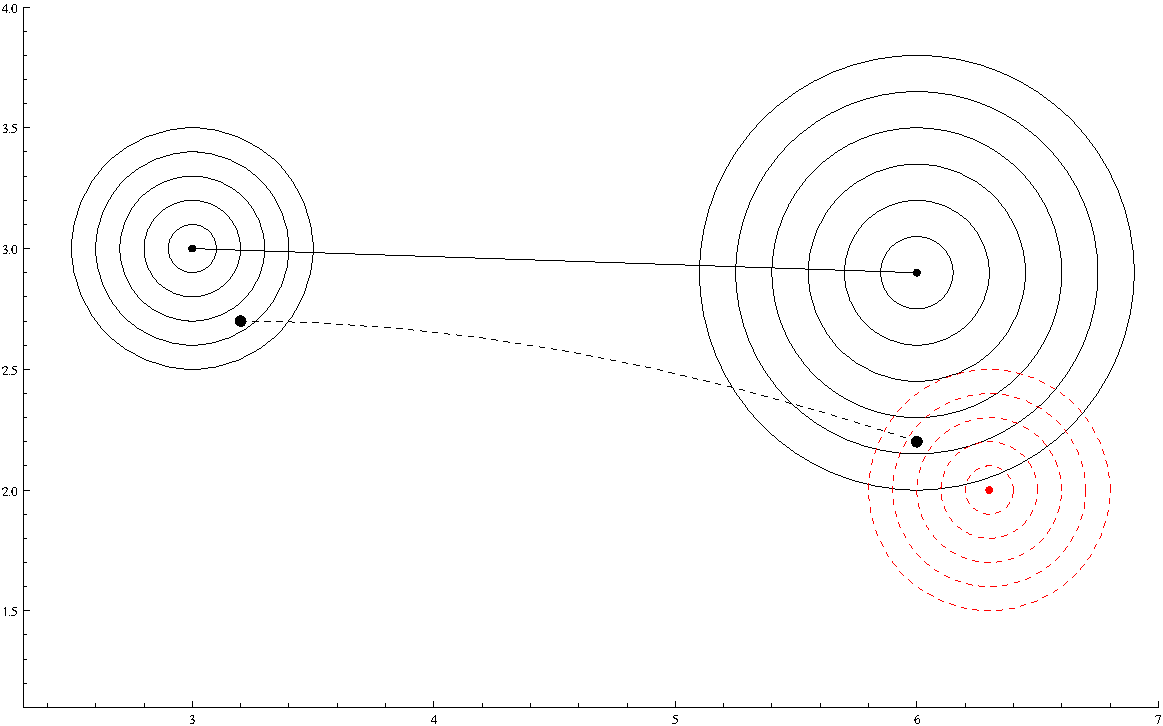
\includegraphics[width=11cm]{enkf5.pdf}};
\node at (65pt,140pt) {$\small \boldsymbol{\psi}^f_{t_0}$};
\node at (78pt,120pt) {$\small \boldsymbol{\psi}^t_{t_0}$};
\node at (255pt,135pt) {$\small \boldsymbol{\psi}^f_{t_1}$};
\node at (255pt,90pt) {$\small \boldsymbol{\psi}^t_{t_1}$};
\node at (278pt,73pt) {$\small \boldsymbol{d}_{t_1}$};
\end{tikzpicture}
\end{figure}

\end{frame}

\begin{frame}{Ensemble Kalman Filter, analyysiongelma 3}

\begin{figure}
\begin{tikzpicture}
\node[above right] (img) at (0,0) {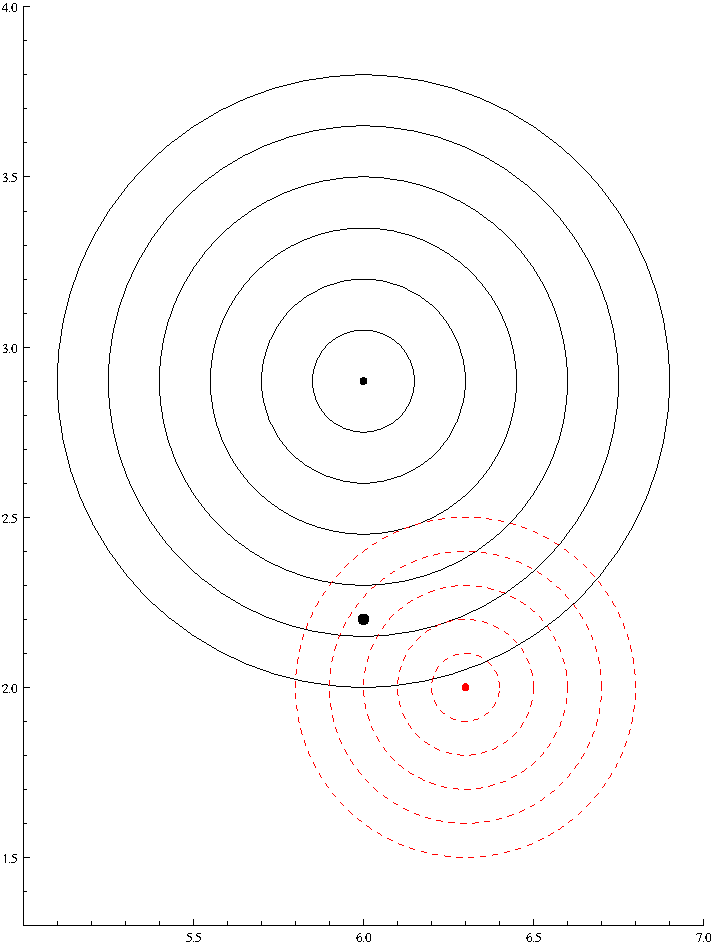
\includegraphics[width=5.5cm]{enkf6.pdf}};
\node at (90pt,137pt) {$\small \boldsymbol{\psi}^f_{t_1}$};
\node at (90pt,85pt) {$\small \boldsymbol{\psi}^t_{t_1}$};
\node at (113pt,68pt) {$\small \boldsymbol{d}_{t_1}$};
\end{tikzpicture}
\end{figure}

\end{frame}

%\begin{frame}{Ensemble Kalman Filter, analyysiongelma 4}

%\begin{figure}
%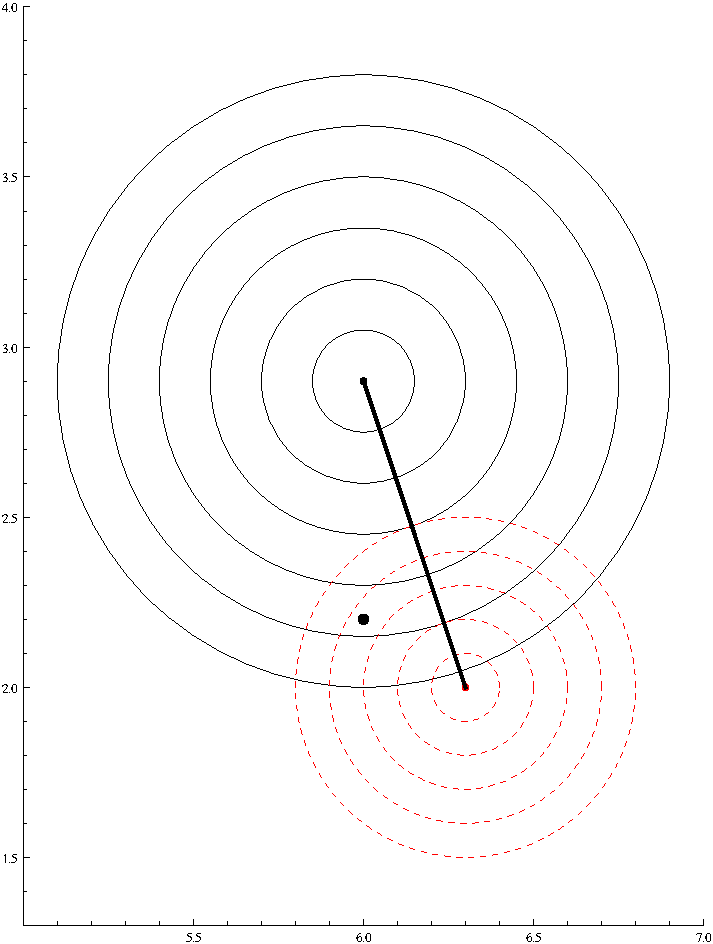
\includegraphics[width=5.5cm]{enkf7.pdf}
%\end{figure}

%\end{frame}

\begin{frame}{Ensemble Kalman Filter, analyysiongelman ratkaisu}

\begin{itemize}
\item \emph{Analysoitu tila} $\boldsymbol{\psi}^a = \boldsymbol{\psi}^f + K\left(\boldsymbol{d}-\boldsymbol{\psi}^f\right)$
\begin{itemize}
\item Jos varianssit samat, $K = \frac{1}{2}$
\item Tässä tapauksessa \[ K = \frac{\sigma_\psi}{\sigma_\psi+\sigma_d} \]
\item Yleisesti \[ \mathbf{K} = \boldsymbol{\Sigma}_\psi\left(\boldsymbol{\Sigma}_\psi+\boldsymbol{\Sigma}_d\right)^{-1} \]
\end{itemize}
\item \pause Jos lisätään vielä mahdollisuus $N > M$, niin 
\[
\boldsymbol{\psi}^a = \boldsymbol{\psi}^f + \boldsymbol{\Sigma}_\psi \mathbf{M}^\mathrm{T} \left(\boldsymbol{\Sigma}_d+\mathbf{M}\boldsymbol{\Sigma}_\psi\mathbf{M}^\mathrm{T}\right)^{-1}\left(\boldsymbol{d}-\mathbf{M}\boldsymbol{\psi}^f\right)
\]
\end{itemize}

\end{frame}

\begin{frame}{Ensemble Kalman Filter, parametrien estimointi}

\begin{itemize}
\item Nyt malli on
\[
\boldsymbol{\dot{\psi}} = \boldsymbol{G}(\boldsymbol{\psi},t;\boldsymbol{\alpha})
\]
\item Käytännössä jatketaan tilaa parametreilla $\boldsymbol{\alpha}$
\[ \boldsymbol{\hat{\psi}}^f = \left(\boldsymbol{\psi}^f,~\boldsymbol{\alpha}\right)^\mathrm{T} \]
\item Karsitaan lisätyt parametrit vertailuista mitattujen arvojen kanssa muokkaamalla mittamatriisia
\item $\rightarrow$ Estimoitavat parametrit loksahtavat kohdalleen ratkaistaessa analyysiongelma
\end{itemize}

\end{frame}

\begin{frame}{Ensemble Kalman Filter, yhteenveto}

\begin{figure}
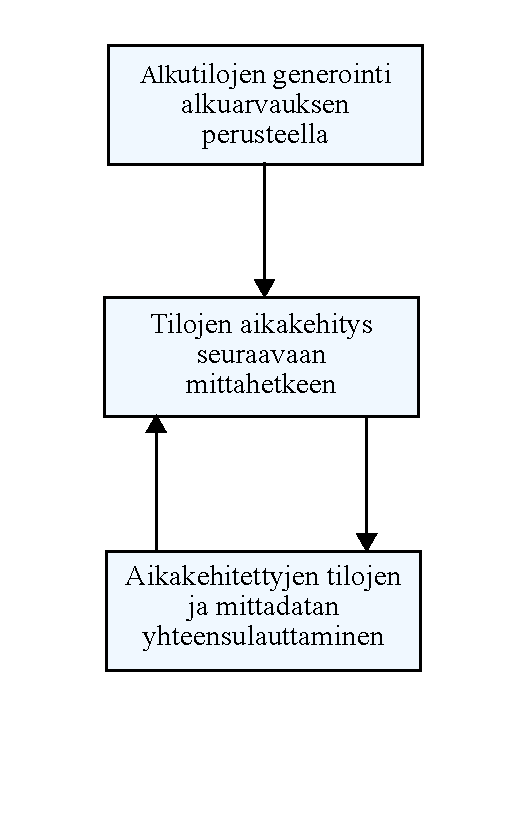
\includegraphics[width=5.5cm]{enkf_luuppi.pdf}
\end{figure}

\end{frame}

\begin{frame}{Takaisin ongelmaan}

\begin{itemize}
\item Malli
\begin{figure}
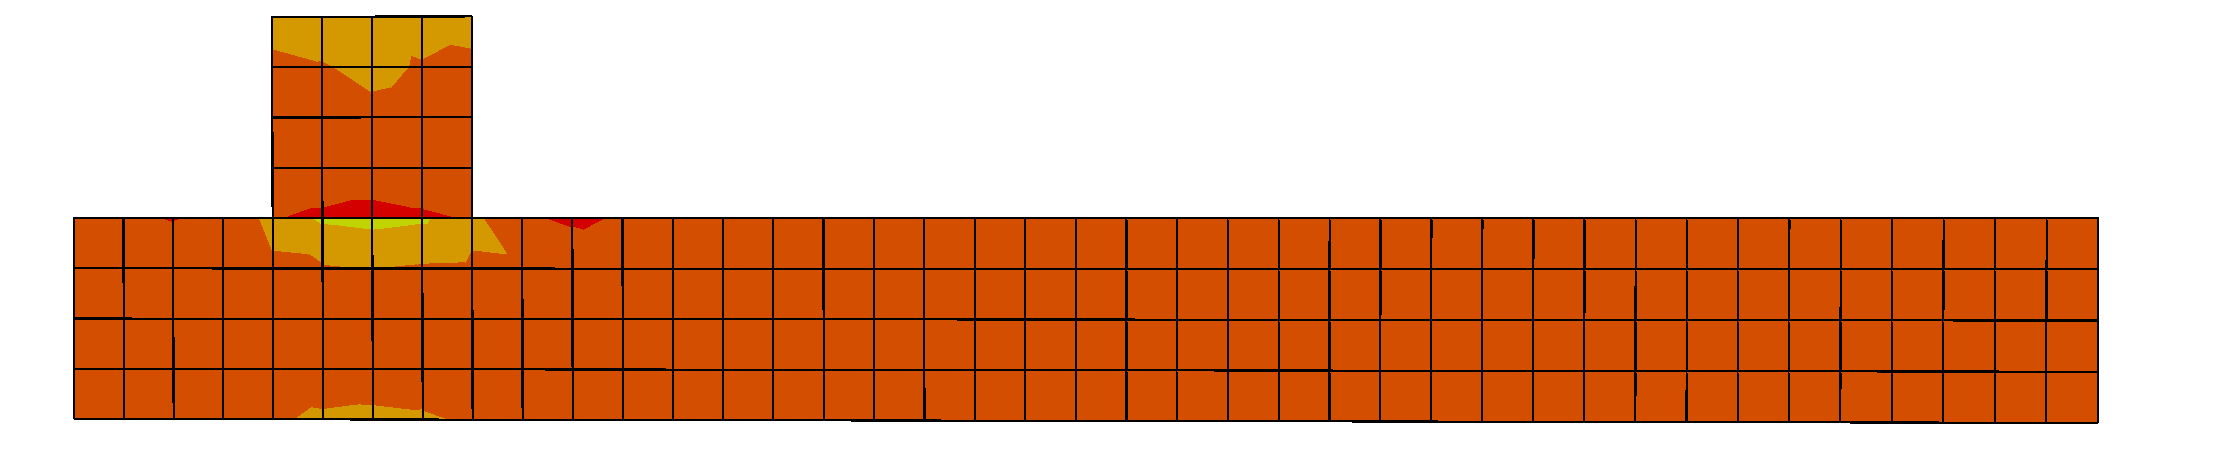
\includegraphics[width=3.3cm]{anim1.pdf}
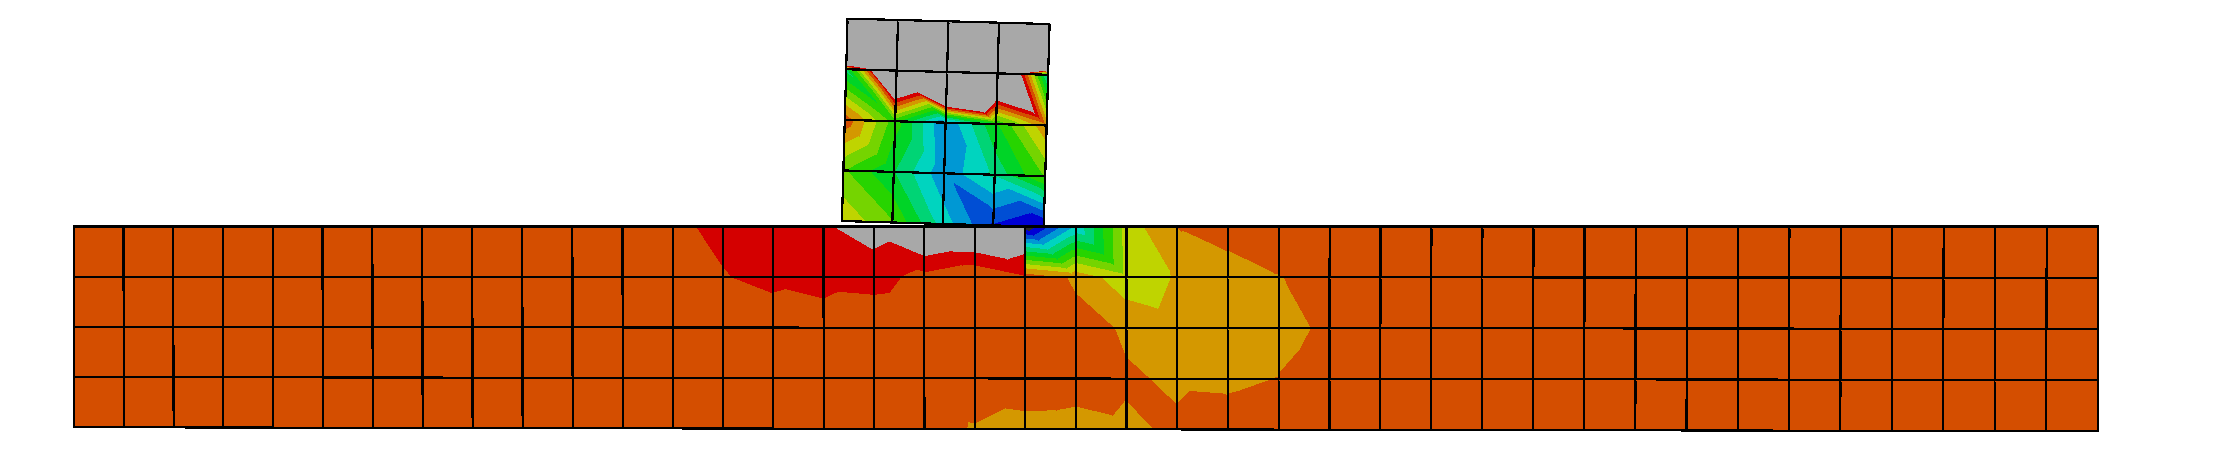
\includegraphics[width=3.3cm]{anim3.pdf}
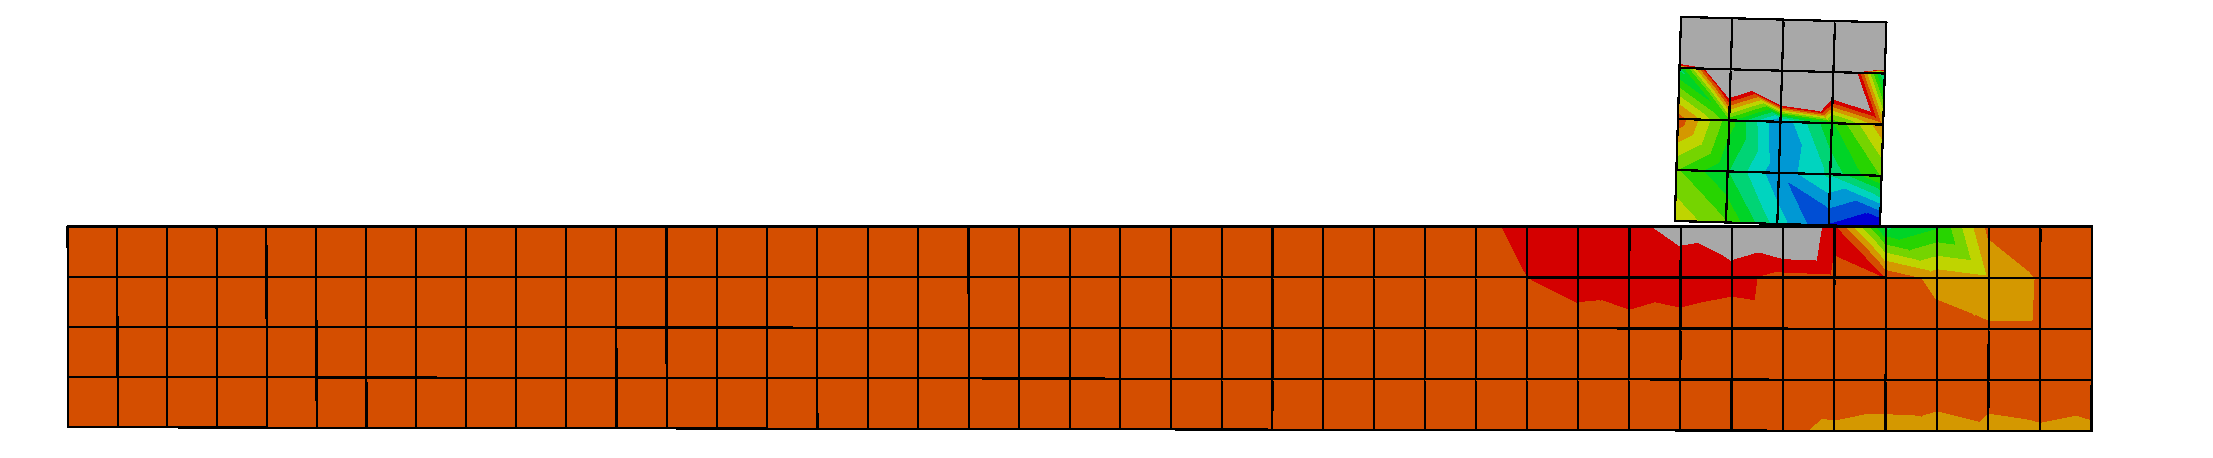
\includegraphics[width=3.3cm]{anim5.pdf}
\end{figure}

\item Estimoitava parametri $\mu$
\item Määritellään tilaksi
\[
  \boldsymbol{\psi} = (\sigma_x^1, \sigma_x^2, \sigma_x^3, \dots, \sigma_x^N, \mu)^\mathrm{T}
\]
\item Alussa ei kosketusta $\Rightarrow$ jännitykset nollia
\item Alkutilan määrää ainoastaan siis $\mu_0$
\end{itemize}

\end{frame}

\begin{frame}{Takaisin ongelmaan 2}

\begin{itemize}
\item Tarvitaan
\begin{itemize}
\item Alkuarvaus $\mu_0=0{,}6$
\item Alkuarvauksen virhe $\sigma_0 = 0{,}1$
\item Kokoelman koko $n=200$
\item Alkukokoelma jakaumasta $\mathcal{N}(\mu_0,\sigma_0^2)$
\end{itemize}
\item Alkukokoelman yksittäinen tila on siis muotoa
\[
\boldsymbol{\psi}_j = (\underbrace{0, 0, \dots, 0, 0,}_{N~\text{kpl}} \mu_0 + \epsilon )^\mathrm{T},~j=1,\dots,n
\]
\item Mitta"hetket": Yläreunan siirtymät $\Delta x = 7,14,21,\dots,70$
\item Mittadata synteettisesti
\end{itemize}

%\begin{itemize}
%\item Alussa ei jännityksiä, joten alkutilan määrää ainoastaan $\mu_0 = 0{,}6$
%\item Oletetaan jokin virhe; tässä $\sigma_0 = 0{,}1$ 
%\item Päätetään kokoelman koko, esim. $n=200$
%\item Generoidaan alkukokoelma jakaumasta $\mathcal{N}(\mu_0,\sigma_0^2)$
%\item Alkukokoelman yksittäinen tila muotoa
%\[
%\boldsymbol{\psi}_j = (\underbrace{0, 0, \dots, 0, 0,}_{N~\text{kpl}} \mu_0 + \epsilon )^\mathrm{T},~j=1,\dots,n
%\]
%\item Mitta"hetket": Yläreunan siirtymä $\Delta x = 7,14,21,\dots,70$
%\item Simuloidaan seuraavaan mittahetkeen asti ja yhteensulautetaan mittaus ja kokoelma $\Rightarrow$ kitkakertoimen estimaatti
%\item Mittahetkiä 10, estimaatteja 10
%\end{itemize}

\end{frame}

\begin{frame}{Synteettisen mittadatan generointi}

\begin{itemize}
\item Minimoidaan inversiorikosta $\rightarrow$ mittadata tiheämmästä verkosta
\end{itemize}

\begin{figure}
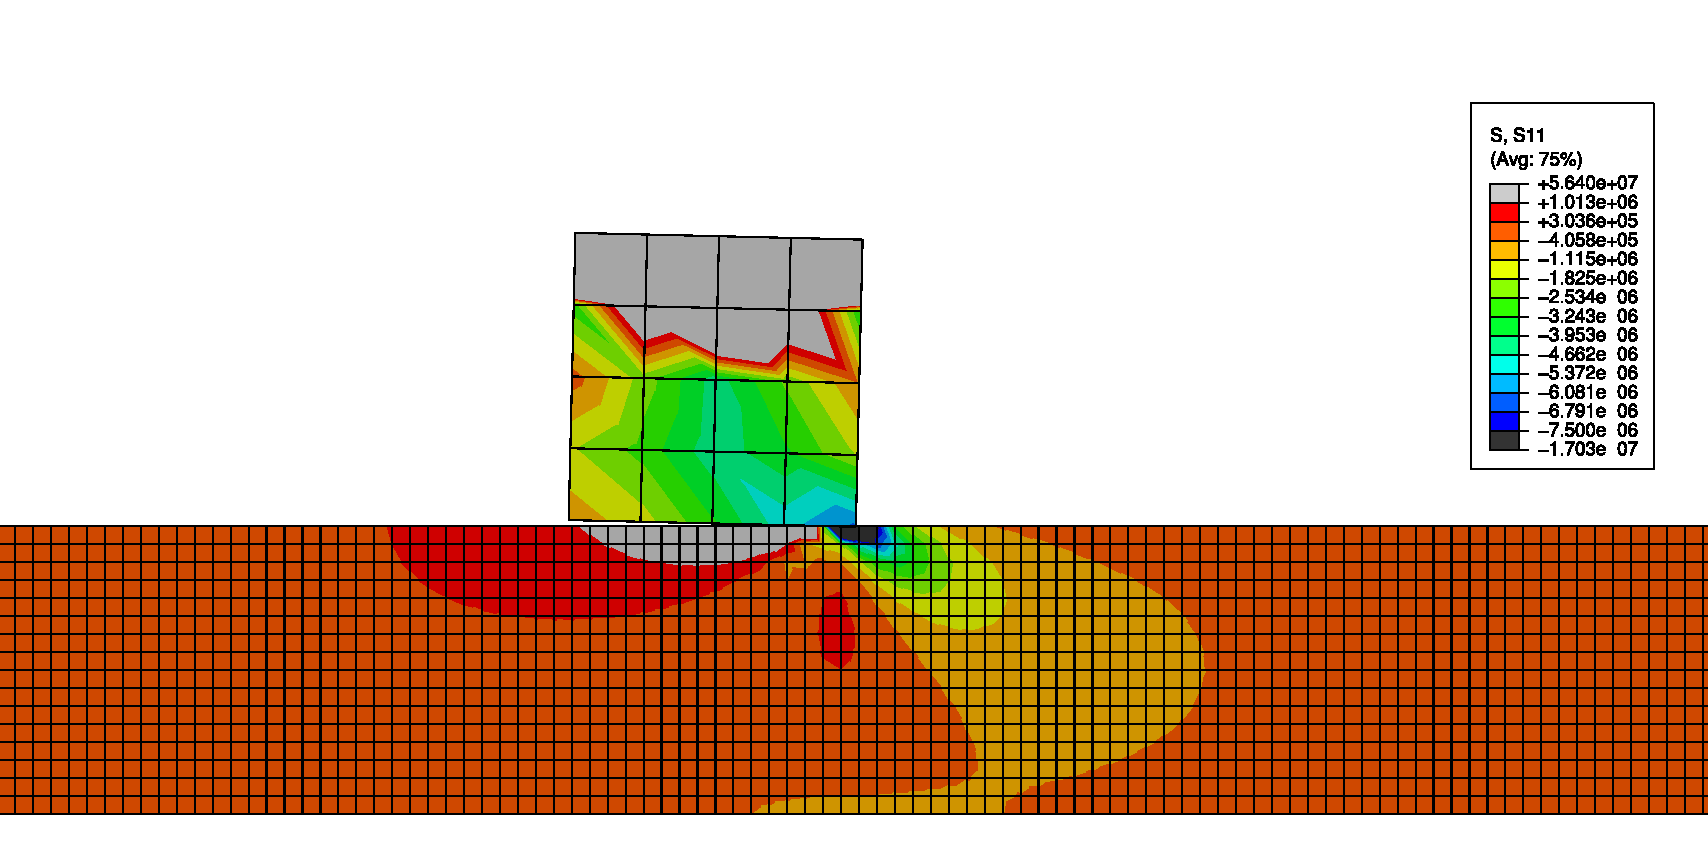
\includegraphics[width=10cm]{finer_mesh.pdf}
\end{figure}

\begin{itemize}
\item Miten verrata tiheämmän ja harvemman verkon antamia jännityksiä?
\end{itemize}

\end{frame}

\begin{frame}{Synteettisen mittadatan generointi 2}

\begin{figure}
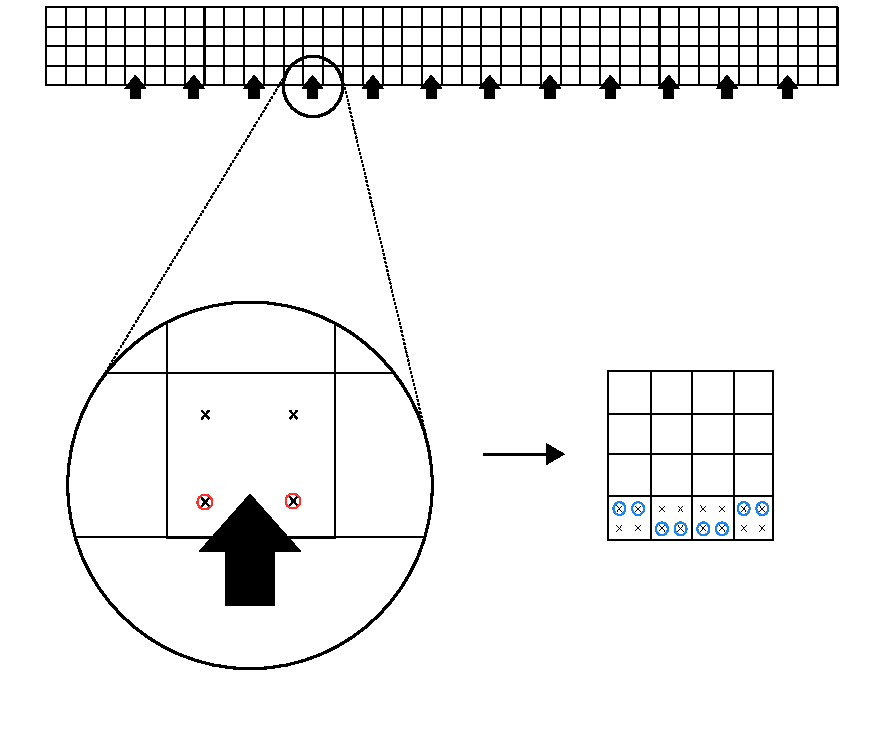
\includegraphics[width=10cm]{fretting_meas_tarkempi.pdf}
\end{figure}

\end{frame}

\begin{frame}{Tuloksia, $\mathbf{Q}=\mathbf{0}$}


\begin{figure}
\begin{tikzpicture}
\node[above right] (img) at (0,0) {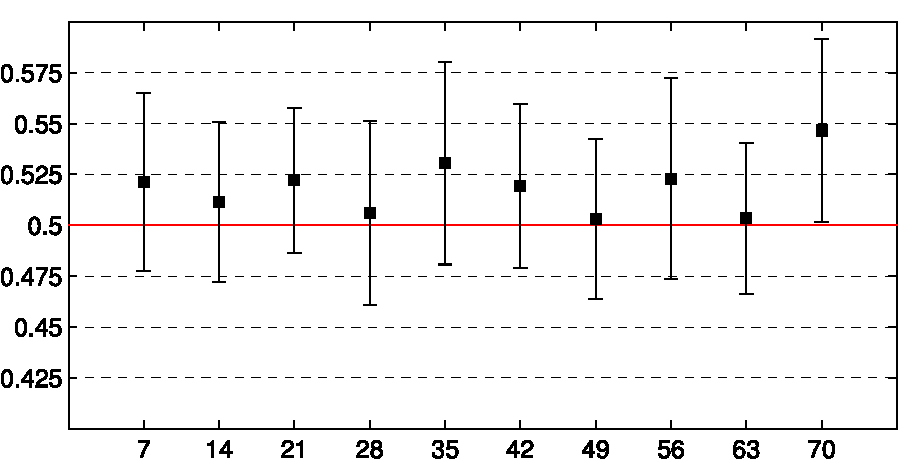
\includegraphics[width=7cm]{xxx_20_no_model_error.pdf}};
\node at (230pt,55pt) {$n=20$};
\end{tikzpicture}
\end{figure}
\vspace{-0.5cm}
\begin{figure}
\begin{tikzpicture}
\node[above right] (img) at (0,0) {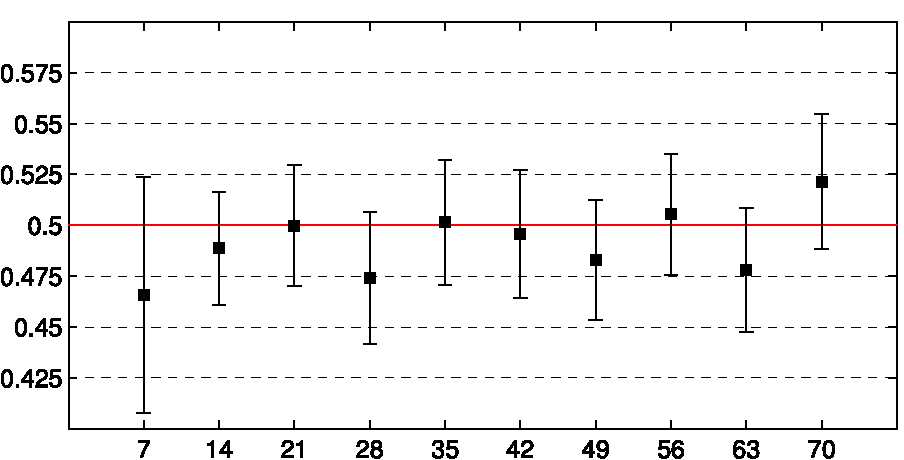
\includegraphics[width=7cm]{xxx_200_no_model_error.pdf}};
\node at (230pt,55pt) {$n=200$};
\end{tikzpicture}
\end{figure} 

\end{frame}

\begin{frame}{Tuloksia, mallivirheen vaikutus, $n=200$}

\begin{figure}
\begin{tikzpicture}
\node[above right] (img) at (0,0) {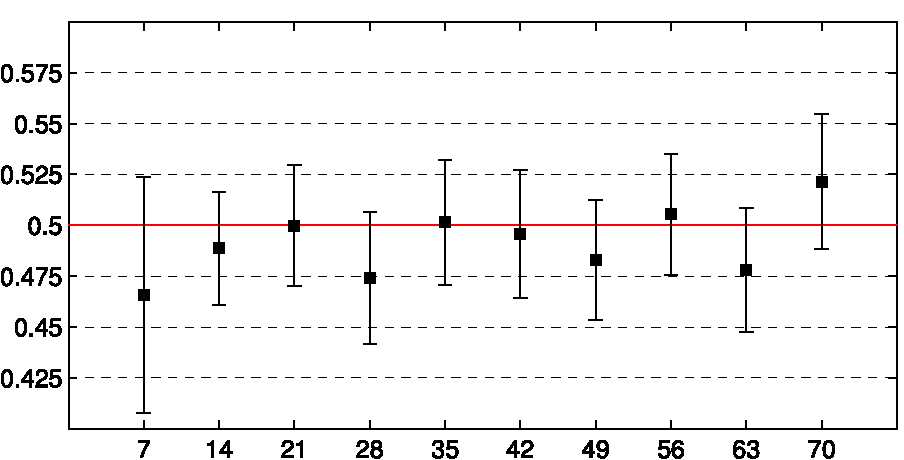
\includegraphics[width=7cm]{xxx_200_no_model_error.pdf}};
\node at (230pt,55pt) {$\mathbf{Q}=\mathbf{0}$};
\end{tikzpicture}
\end{figure}
\vspace{-0.5cm}
\begin{figure}
\begin{tikzpicture}
\node[above right] (img) at (0,0) {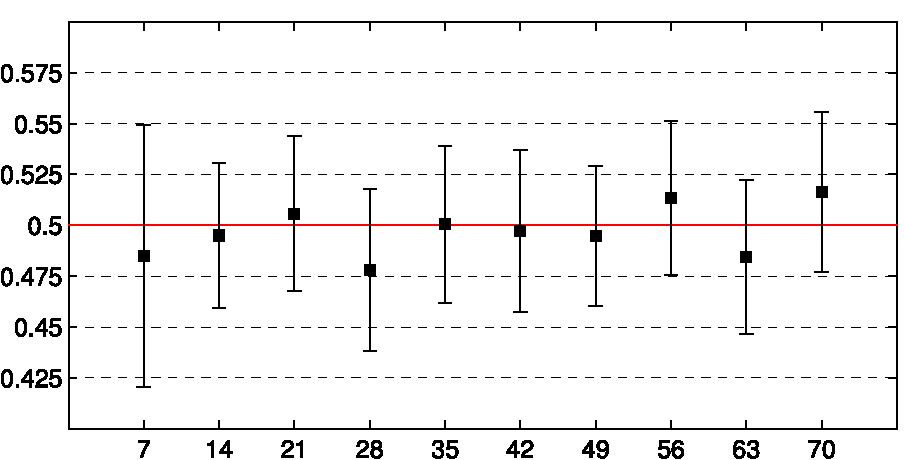
\includegraphics[width=7cm]{xxx_200_model_error.pdf}};
\node at (230pt,55pt) {$\mathbf{Q}=\mathbf{I}\sigma$};
\end{tikzpicture}
\end{figure} 

%\begin{figure}
%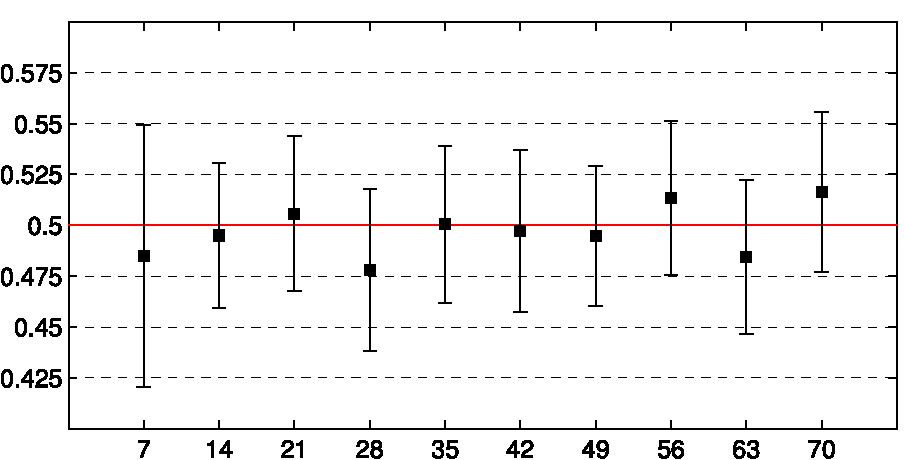
\includegraphics[width=7cm]{xxx_200_model_error.pdf}
%\end{figure}

%\begin{figure}
%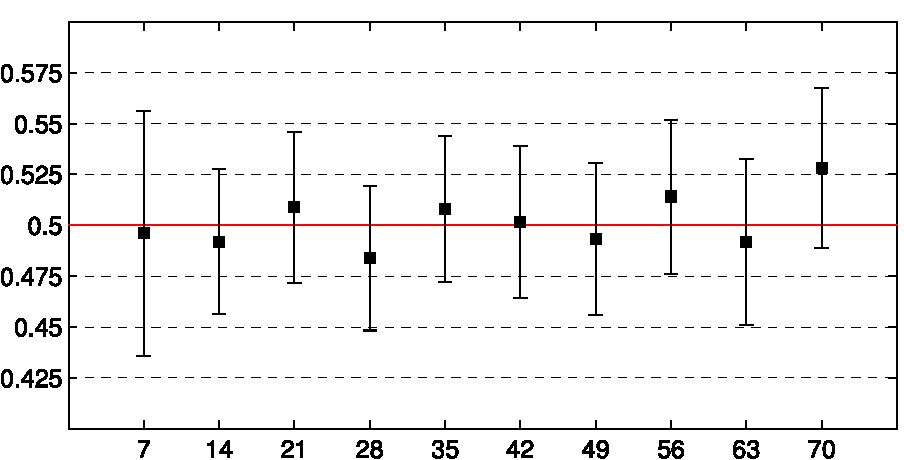
\includegraphics[width=7cm]{xxx_1000_model_error.pdf}
%\end{figure}

\end{frame}

\begin{frame}{Kokoelman koon vaikutus, keskiarvo}

Punainen: $\Delta x=70$, sininen: $\Delta x=42$, vihreä: $\Delta x=14$

\begin{figure}
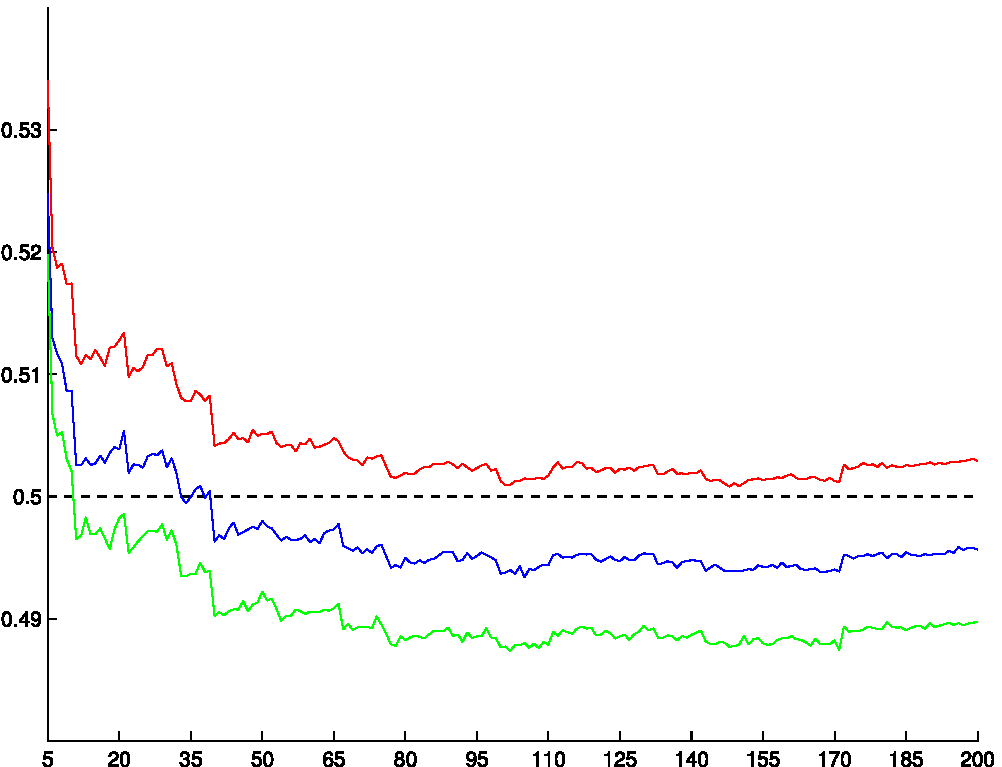
\includegraphics[width=9cm]{mean_conv_2_6_10.pdf}
\end{figure}

\end{frame}

\begin{frame}{Kokoelman hajonta}

\begin{figure}
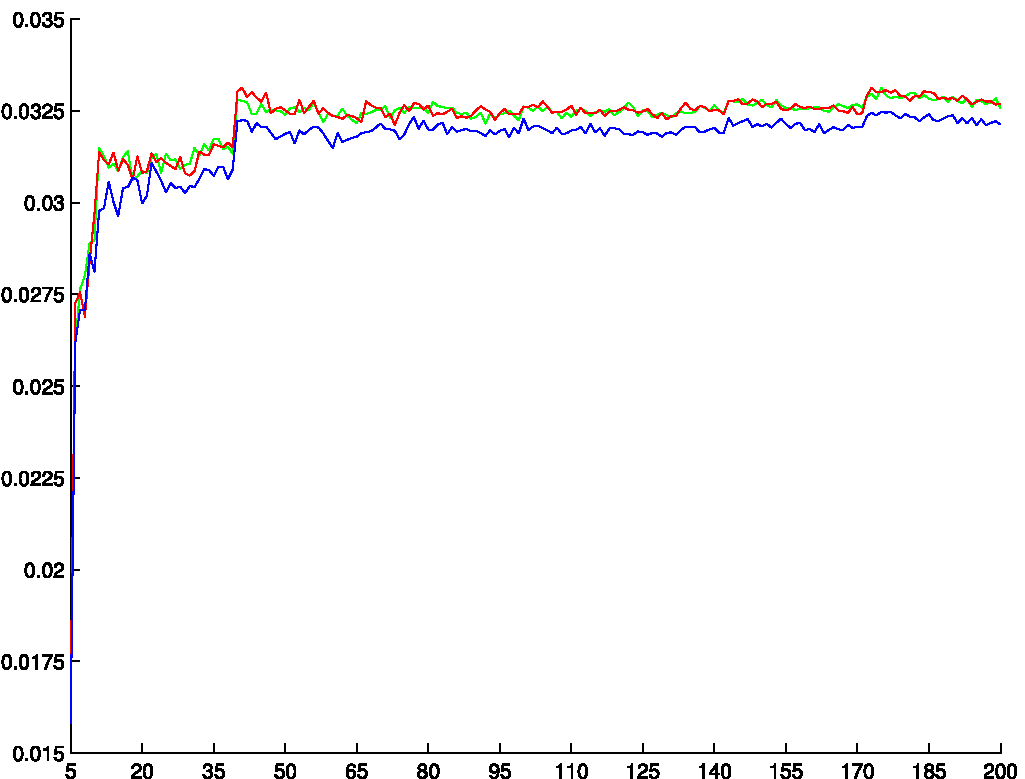
\includegraphics[width=9cm]{ensemble_stdev.pdf}
\end{figure}

\end{frame}

\begin{frame}{Peräkkäisten analyysien varianssi}

\begin{figure}
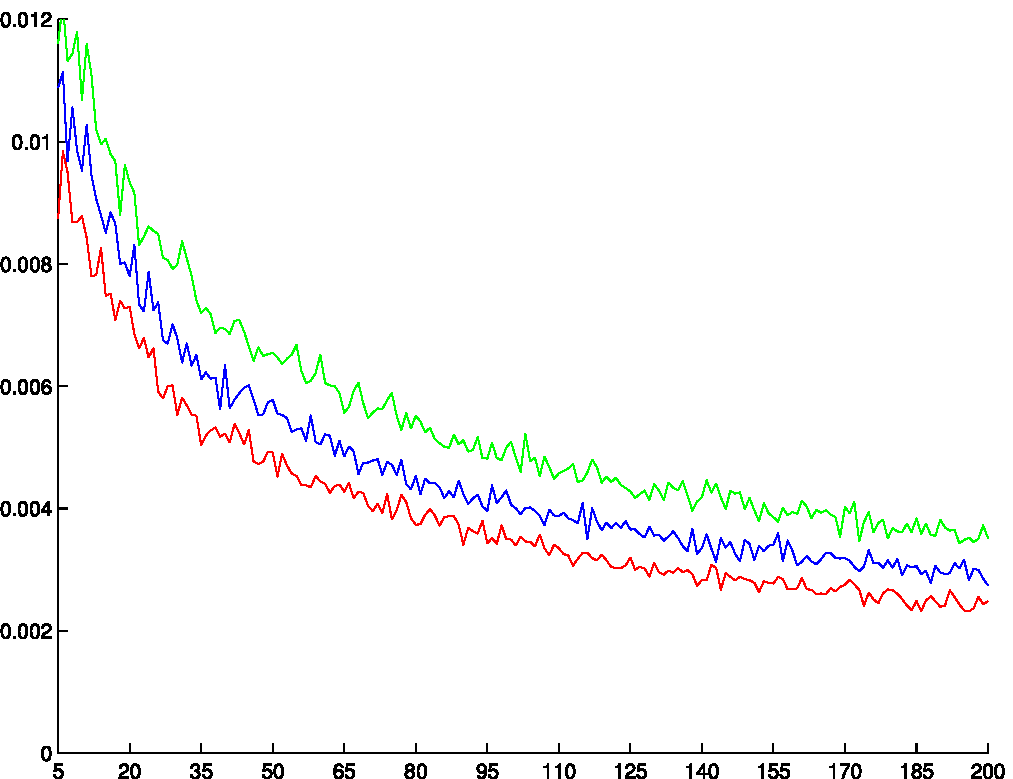
\includegraphics[width=9cm]{stdev_between_analysis.pdf}
\end{figure}

\end{frame}

\begin{frame}{Kysymyksiä?}


\end{frame}

\end{document}
